\section{覆叠空间}
\label{section:ch09-sec53}

我们已经指出 $\mathbb{R}^{n}$ 的任何凸子空间的基本群都是平凡群, 现在来计算非平凡的基本群. 计算基本群最有效的工具之一便是覆叠空间的概念, 我们将在这一节中介绍. 覆叠空间在 Riemann 曲面和复流形的研究中也是很重要的. (见 [A-S].) 我们将在第 13 章中进行更为详细的研究.

\begin{definition}[均衡覆盖与覆叠映射]
\label{definition:ch09-sec53-covering}
设 $p\colon E\to B$ 是一个连续的满射, $U$ 是 $B$ 的开集. 如果 $U$ 的原像 $p^{-1}(U)$ 能够表示为 $E$ 中一些占有最广位置的开集 $V_\alpha$ 的并, 并且对于每一个 $\alpha$, 将 $p$ 限制在 $V_\alpha$ 上都是从 $V_\alpha$ 到 $U$ 上的同胚, 则称 $p$ \textbf{均衡地覆盖}(evenly covered) $U$. 集族 $\{V_\alpha\}$ 称为 $p^{-1}(U)$ 的一个\textbf{片状分拆}(partition into slice).

如果 $U$ 是被 $p$ 均衡地覆盖着的开集, 我们常将集合 $p^{-1}(U)$ 画成"一叠薄饼"悬在 $U$ 的上方, 每一片"薄饼"都和 $U$ 的大小形状相同. 而映射 $p$ 则把它们挤压到 $U$ 上 (见图 \cref{figure:ch09-fig-53-1}). 注意, 如果 $U$ 被 $p$ 均衡地覆盖, 而 $W$ 是包含于 $U$ 的一个开集, 那么 $W$ 也被 $p$ 均衡地覆盖.

设 $p\colon E\to B$ 为连续的满射. 如果 $B$ 的每一个点 $b$ 有邻域 $U$ 被 $p$ 均衡地覆盖着, 则 $p$ 称为\textbf{覆叠映射}(covering map), $E$ 称为 $B$ 的\textbf{覆叠空间}(covering space).
\end{definition}

\par
\begin{figure}[htbp]
\centering
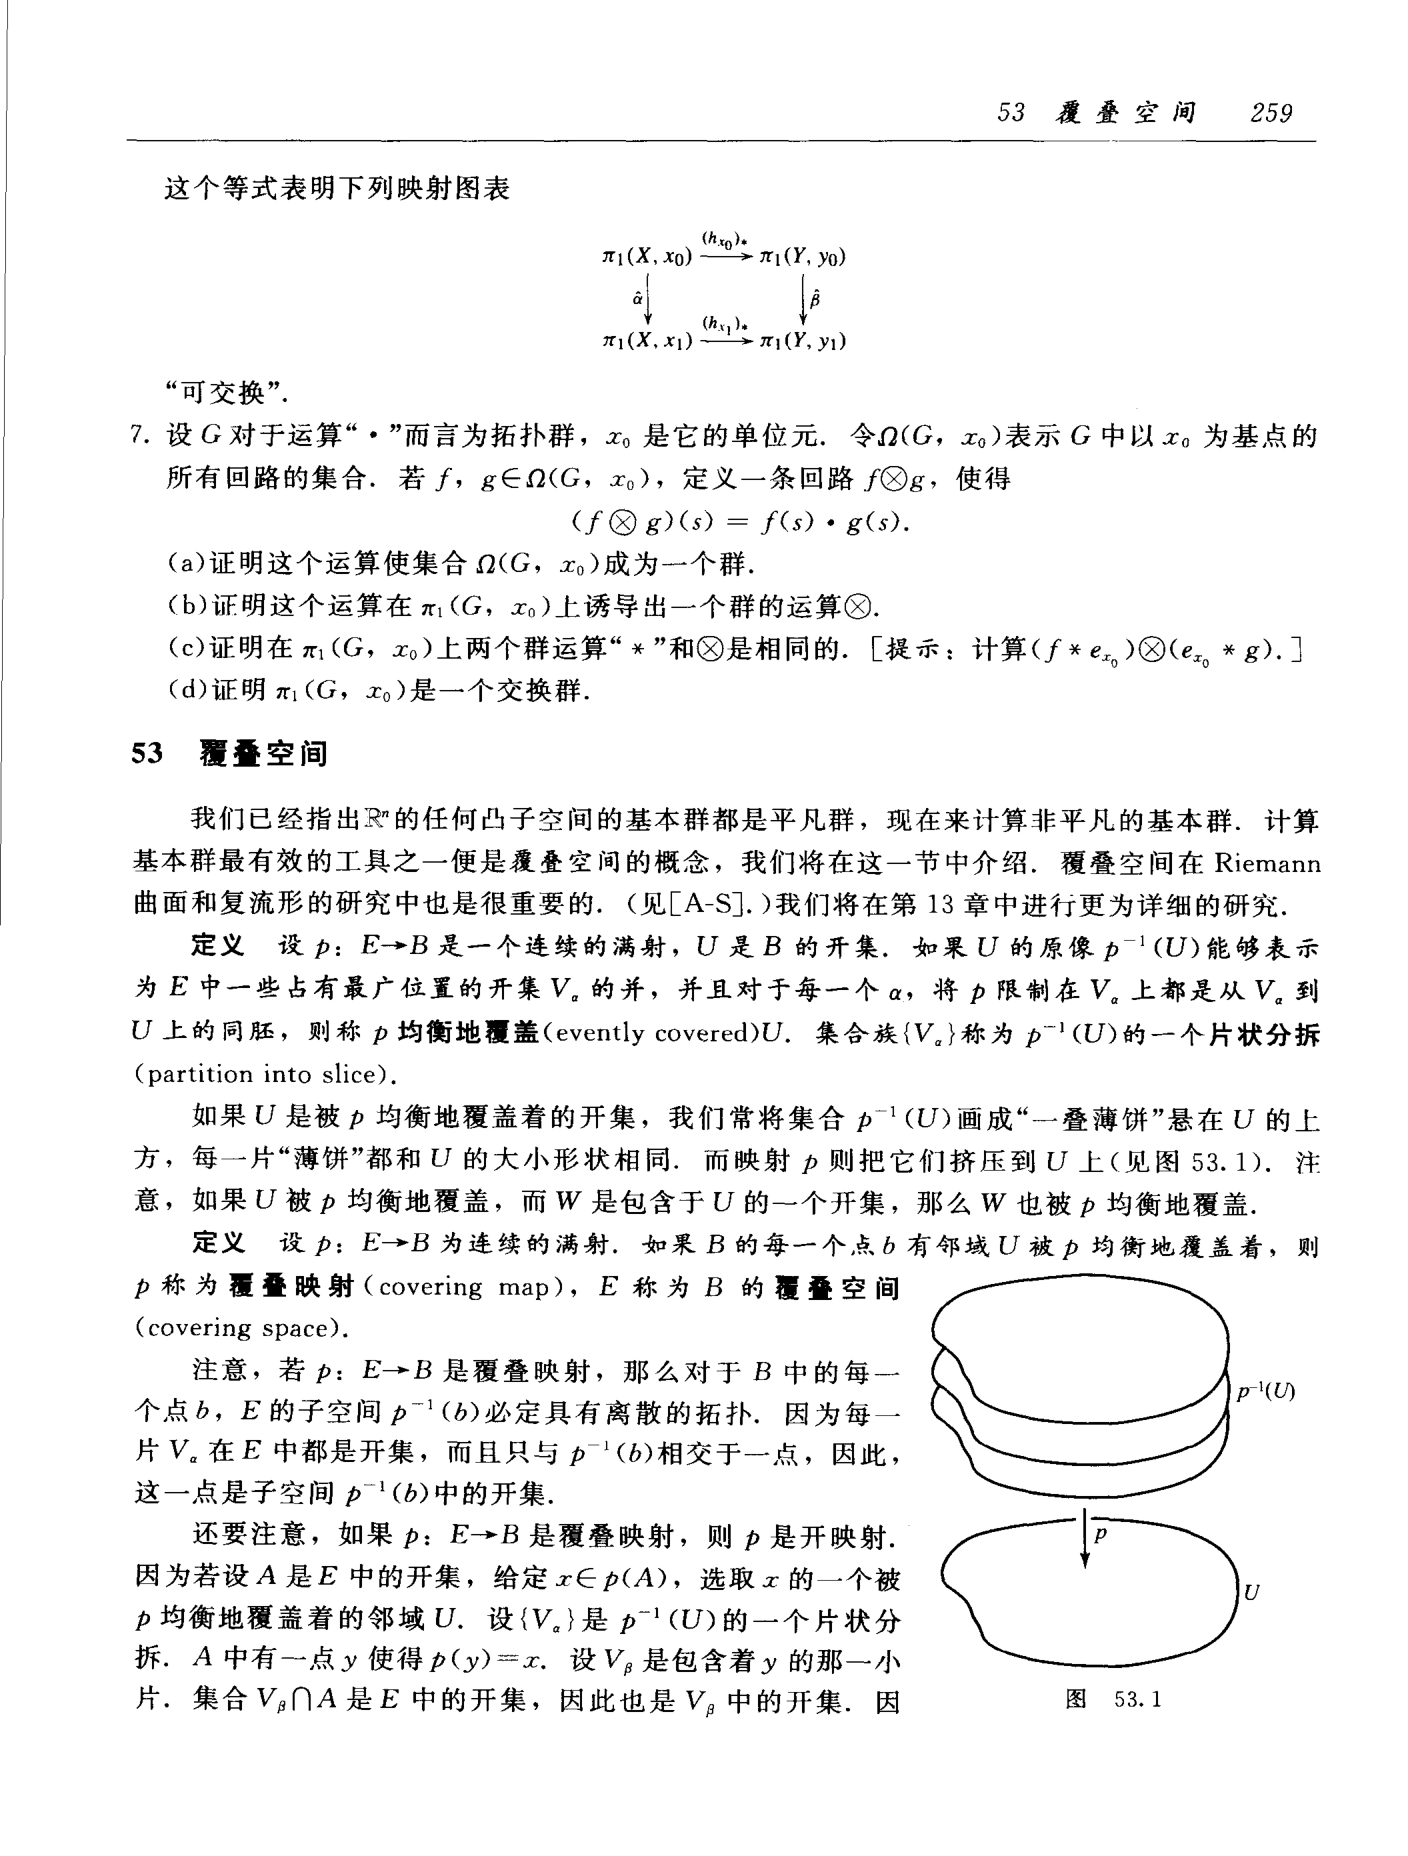
\includegraphics[width=0.4\textwidth]{image/fig-53-1.png}
\caption{均衡覆盖.}
\label{figure:ch09-fig-53-1}
\end{figure}

注意, 若 $p\colon E\to B$ 是覆叠映射, 那么对于 $B$ 中的每一个点 $b$, $E$ 的子空间 $p^{-1}(b)$ 必定具有离散的拓扑. 因为每一片 $V_\alpha$ 在 $E$ 中都是开集, 而且只与 $p^{-1}(b)$ 相交于一点, 因此, 这一点是子空间 $p^{-1}(b)$ 中的开集.

还要注意, 如果 $p\colon E\to B$ 是覆叠映射, 则 $p$ 是开映射. 因为若设 $A$ 是 $E$ 中的开集, 给定 $x\in p(A)$, 选取 $x$ 的一个被 $p$ 均衡地覆盖着的邻域 $U$. 设 $\{V_\alpha\}$ 是 $p^{-1}(U)$ 的一个片状分拆. $A$ 中有一点 $y$ 使得 $p(y)=x$. 设 $V_\beta$ 是包含着 $y$ 的那一小片. 集合 $V_\beta\cap A$ 是 $E$ 中的开集, 因此也是 $V_\beta$ 中的开集. 因为 $p$ 将 $V_\beta$ 同胚地映到 $U$ 上, 集合 $p(V_\beta\cap A)$ 是 $U$ 中的开集, 因此也是 $B$ 中的开集. 于是 $p(V_\beta\cap A)$ 是 $x$ 的一个包含在 $p(A)$ 中的邻域, 这便是我们要证明的.

\begin{example}
\label{example:ch09-sec53-1}
设 $X$ 是一个空间, $i\colon X\to X$ 为恒等映射, 那么 $i$ 便是 (最简单的) 覆叠映射. 更一般地, 设 $E$ 是由 $X$ 的 $n$ 个占有最广位置的"副本"组成的空间 $X\times\{1,\cdots,n\}$. 映射 $p\colon E\to X$ 定义为对于所有的 $i$, $p(x,i)=x$, 则 $p$ 也是一个 (相当简单的) 覆叠映射. 对于这种情形, 我们可以将整个空间 $E$ 画成 $X$ 上方的一叠薄饼.

为了避开这类简单的叠饼式覆叠空间, 我们常要求覆叠空间是道路连通的. 这样一个非平凡覆叠空间的例子如下.
\end{example}

\begin{theorem}
\label{theorem:ch09-sec53-53-1}
设映射 $p\colon\mathbb{R}\to S^{1}$ 定义为
\[
p(x)=(\cos 2\pi x,\sin 2\pi x),
\]
则 $p$ 是一个覆叠映射.
\end{theorem}

\par
\begin{figure}[htbp]
\centering
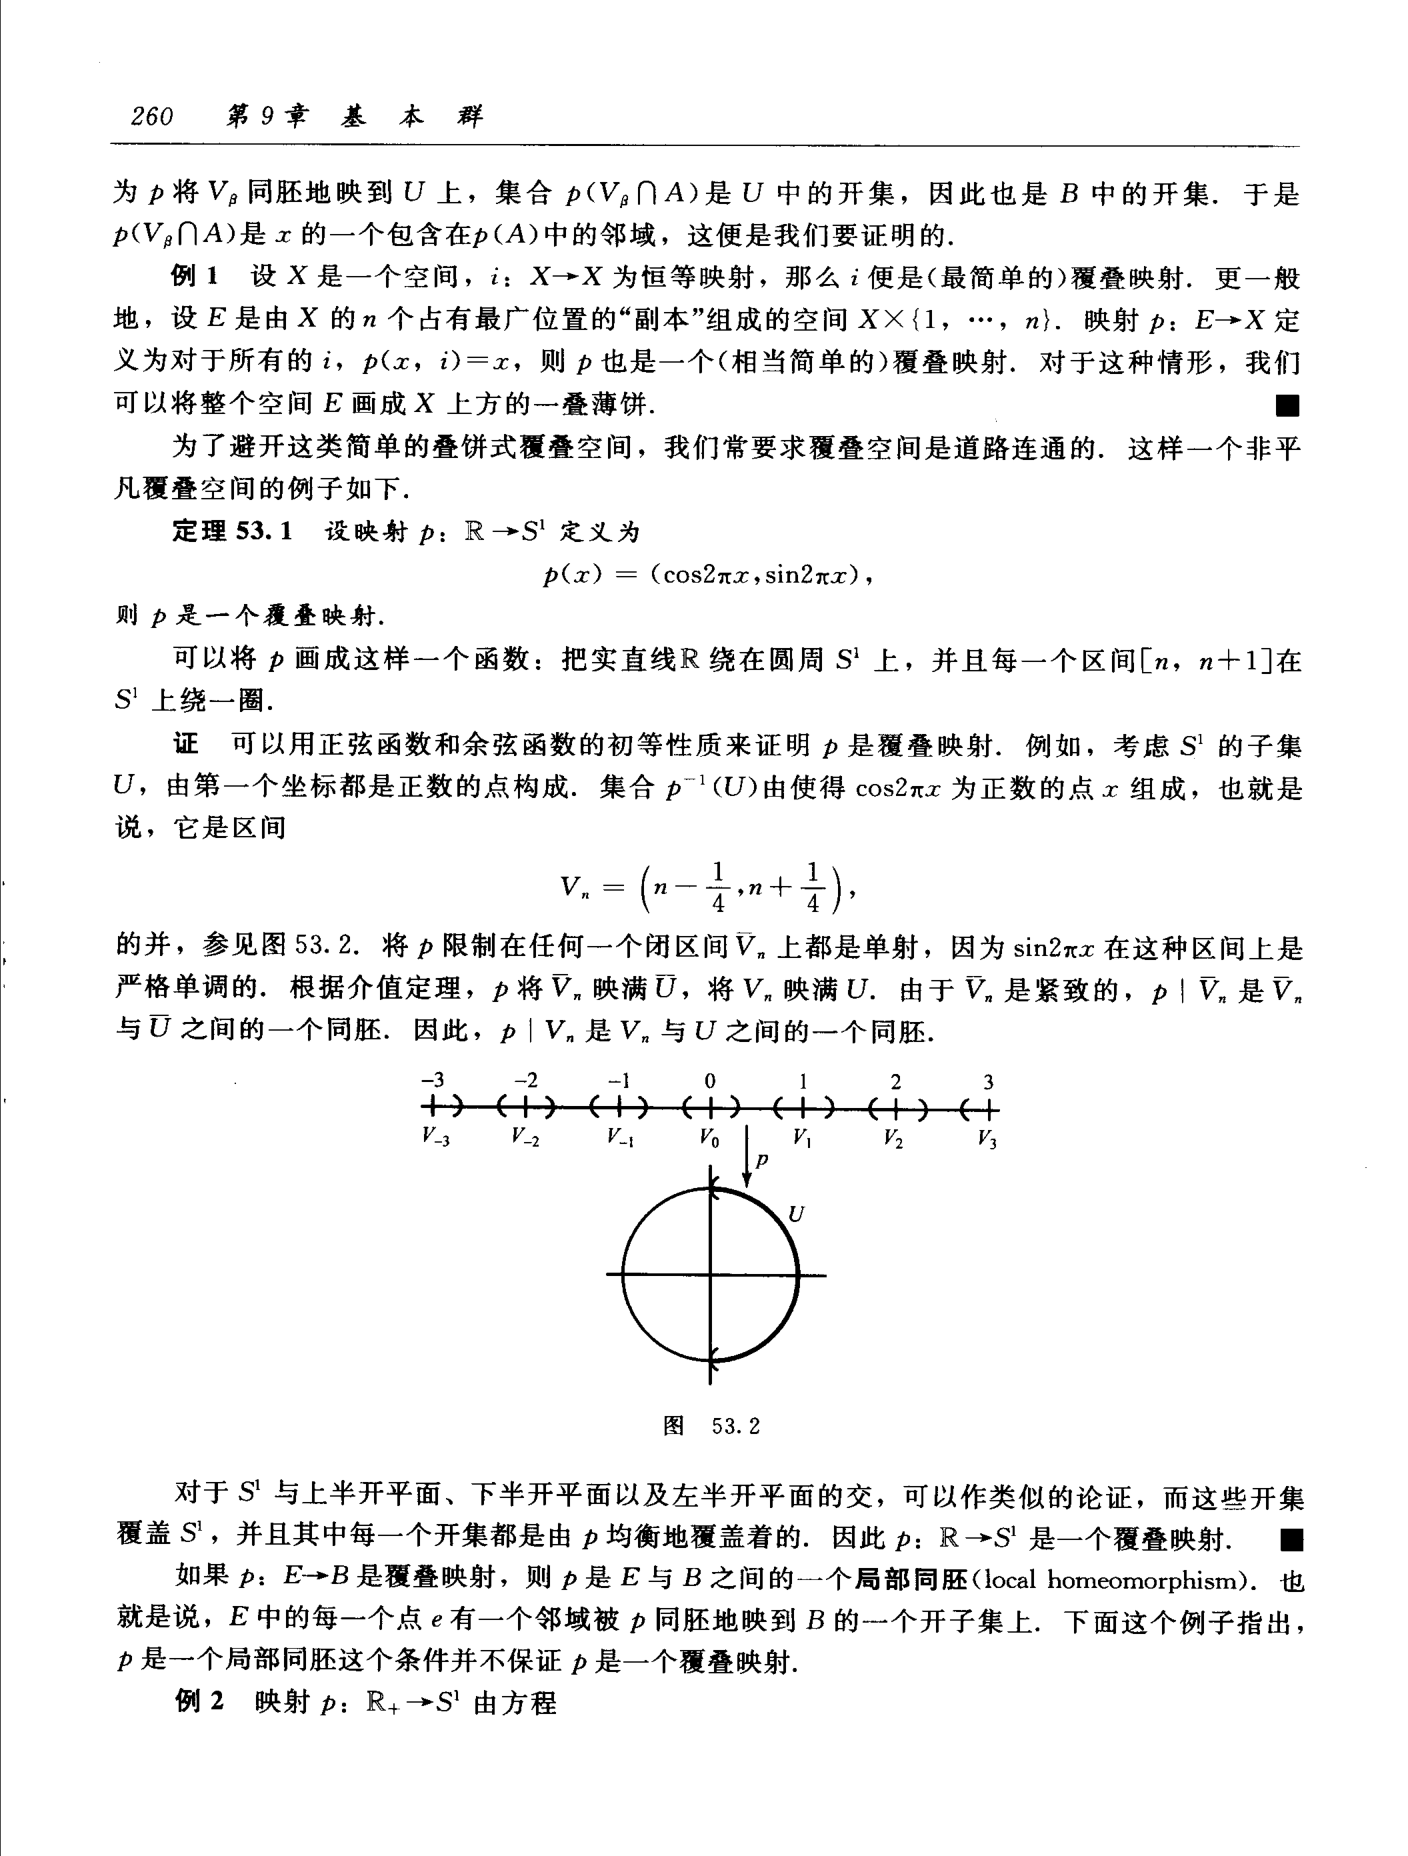
\includegraphics[width=0.7\textwidth]{image/fig-53-2.png}
\caption{$p\colon\mathbb{R}\to S^{1}$.}
\label{figure:ch09-fig-53-2}
\end{figure}

\begin{proof}
可以将 $p$ 画成这样一个函数: 把实直线 $\mathbb{R}$ 绕在圆周 $S^{1}$ 上, 并且每一个区间 $[n,n+1]$ 在 $S^{1}$ 上绕一圈.

可以用正弦函数和余弦函数的初等性质来证明 $p$ 是覆叠映射. 例如, 考虑 $S^{1}$ 的子集 $U$, 由第一个坐标都是正数的点构成. 集合 $p^{-1}(U)$ 由使得 $\cos 2\pi x$ 为正数的点 $x$ 组成, 也就是说, 它是区间
\[
V_{n}=\left(n-\frac{1}{4},n+\frac{1}{4}\right)
\]
的并, 参见图 \cref{figure:ch09-fig-53-2}. 将 $p$ 限制在任何一个闭区间 $\overline{V}_n$ 上都是单射, 因为 $\sin 2\pi x$ 在这种区间上是严格单调的. 根据介值定理, $p$ 将 $\overline{V}_n$ 映满 $\overline{U}$, 将 $V_n$ 映满 $U$. 由于 $\overline{V}_n$ 是紧致的, $p\mid\overline{V}_n$ 是 $\overline{V}_n$ 与 $\overline{U}$ 之间的一个同胚. 因此, $p\mid V_n$ 是 $V_n$ 与 $U$ 之间的一个同胚.


对于 $S^{1}$ 与上半开平面、下半开平面以及左半开平面的交, 可以作类似的论证, 而这些开集覆盖 $S^{1}$, 并且其中每一个开集都是由 $p$ 均衡地覆盖着的. 因此 $p\colon\mathbb{R}\to S^{1}$ 是一个覆叠映射.
\end{proof}

如果 $p\colon E\to B$ 是覆叠映射, 则 $p$ 是 $E$ 与 $B$ 之间的一个\textbf{局部同胚}(local homeomorphism). 也就是说, $E$ 中的每一个点 $e$ 有一个邻域被 $p$ 同胚地映到 $B$ 的一个开子集上. 下面这个例子指出, $p$ 是一个局部同胚这个条件并不保证 $p$ 是一个覆叠映射.

\begin{example}
\label{example:ch09-sec53-2}
映射 $p\colon\mathbb{R}_{+}\to S^{1}$ 由方程
\[
p(x)=(\cos 2\pi x,\sin 2\pi x)
\]
定义. 这个映射是一个满射, 也是一个局部同胚. 参见图 \cref{figure:ch09-fig-53-3}. 然而它并不是覆叠映射, 因为点 $b_0=(1,0)$ 没有一个邻域 $U$ 被 $p$ 均衡地覆盖. $b_0$ 的典型邻域 $U$ 的逆像由每一个正整数 $n>0$ 的一个邻域 $V_n$ 和一个形如 $(0,\varepsilon)$ 的小区间 $V_0$ 构成. 每一个区间 $V_n$ ($n>0$) 被 $p$ 同胚地映到 $U$ 上, 然而区间 $V_0$ 却仅仅由 $p$ 嵌入到 $U$ 中.
\end{example}

\par
\begin{figure}[htbp]
\centering
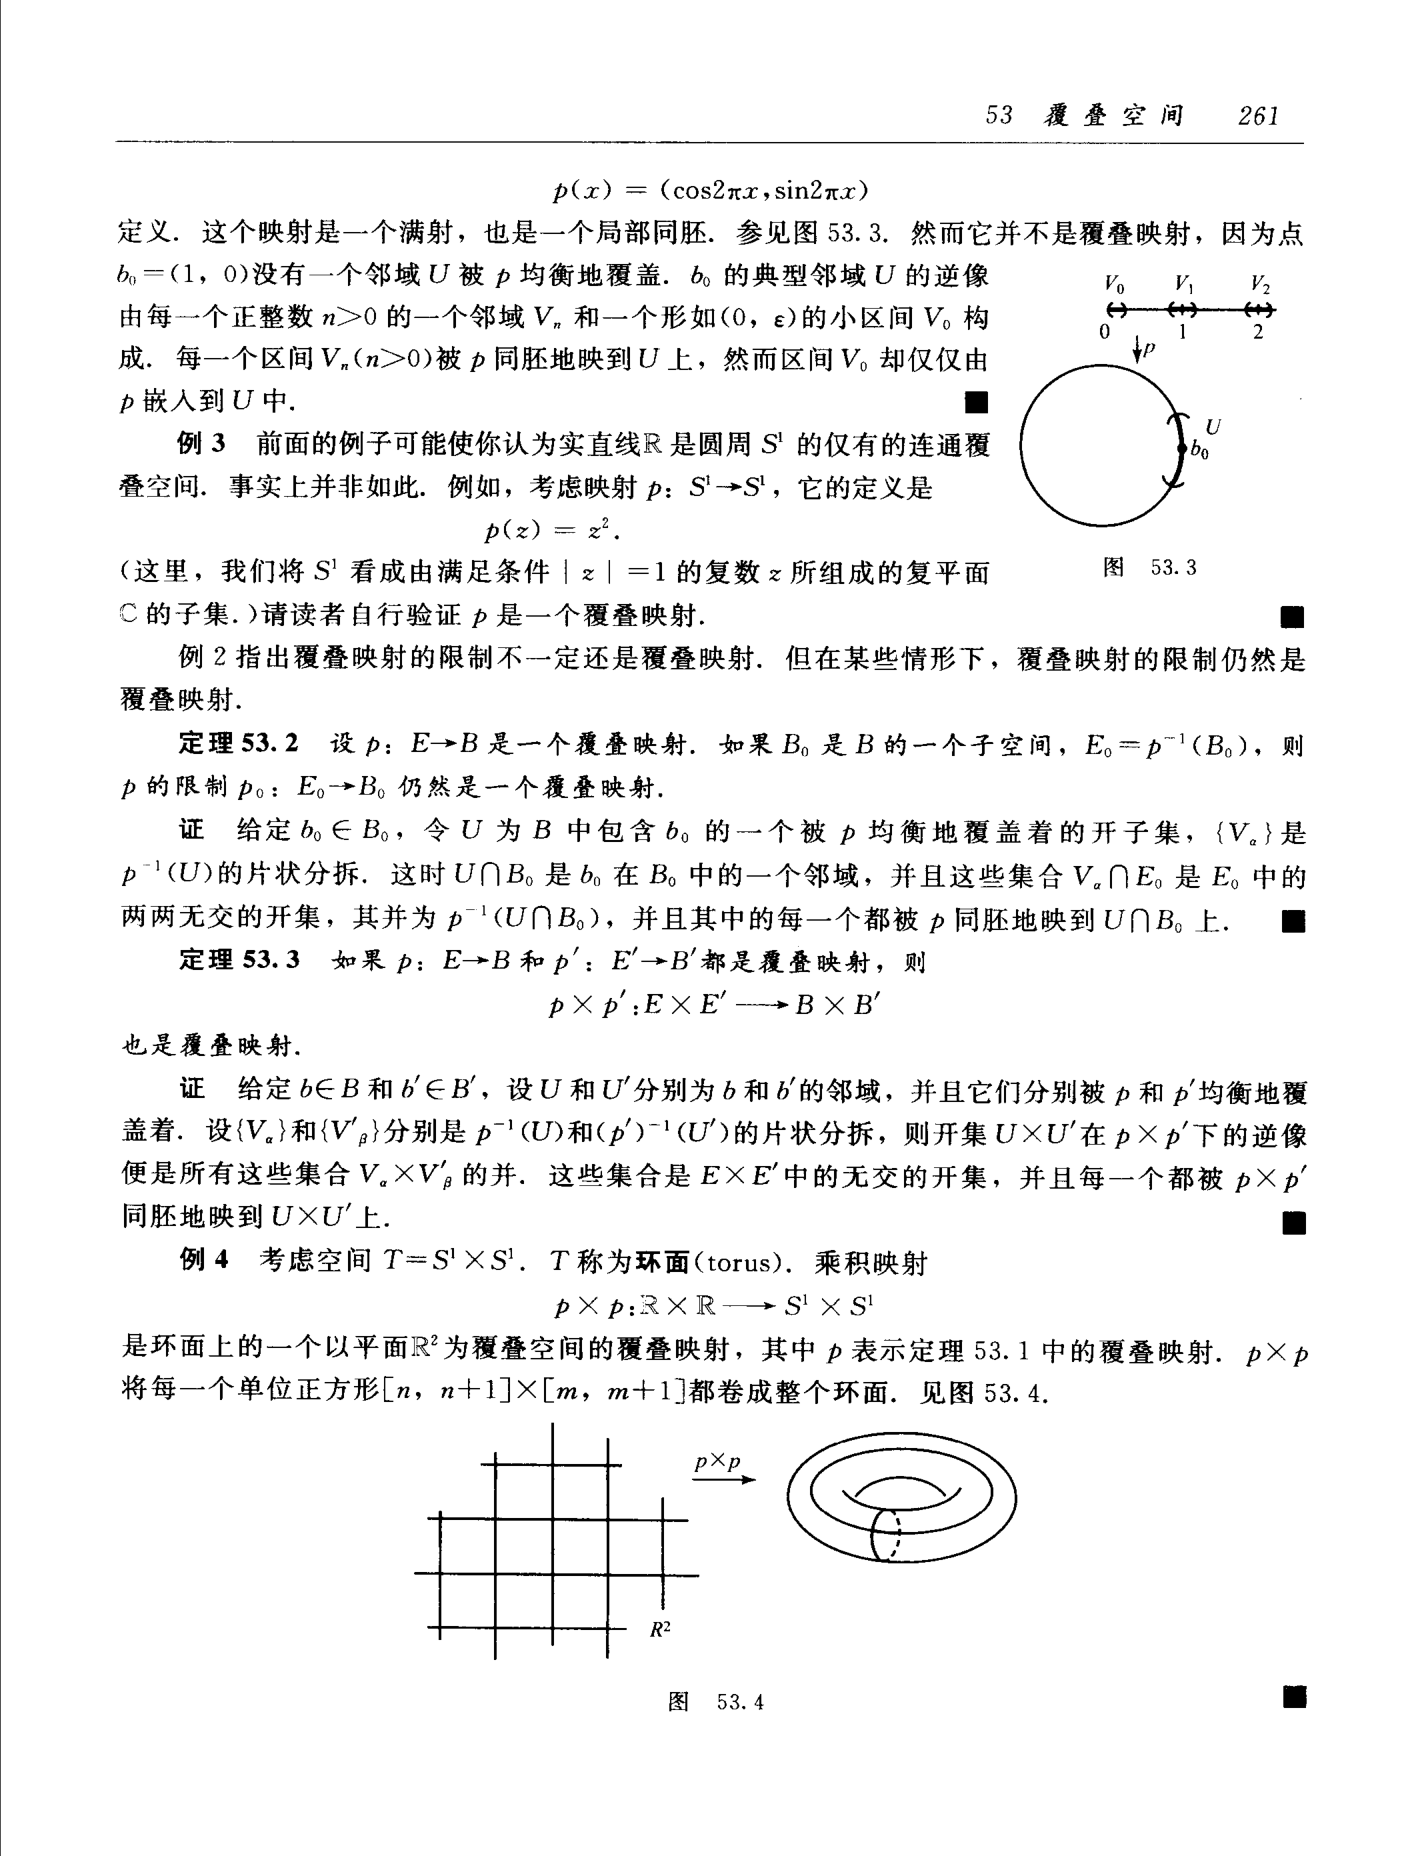
\includegraphics[width=0.5\textwidth]{image/fig-53-3.png}
\caption{$p\colon\mathbb{R}_{+}\to S^{1}$.}
\label{figure:ch09-fig-53-3}
\end{figure}

\begin{example}
\label{example:ch09-sec53-3}
前面的例子可能使你认为实直线 $\mathbb{R}$ 是圆周 $S^{1}$ 的仅有的连通覆叠空间. 事实上并非如此. 例如, 考虑映射 $p\colon S^{1}\to S^{1}$, 它的定义是
\[
p(z)=z^{2}.
\]
(这里, 我们将 $S^{1}$ 看成由满足条件 $|z|=1$ 的复数 $z$ 所组成的复平面 $\mathbb{C}$ 的子集.) 请读者自行验证 $p$ 是一个覆叠映射.
\end{example}

例 2 指出覆叠映射的限制不一定还是覆叠映射. 但在某些情形下, 覆叠映射的限制仍然是覆叠映射.

\begin{theorem}
\label{theorem:ch09-sec53-53-2}
设 $p\colon E\to B$ 是一个覆叠映射. 如果 $B_0$ 是 $B$ 的一个子空间, $E_0=p^{-1}(B_0)$, 则 $p$ 的限制 $p_0\colon E_0\to B_0$ 仍然是一个覆叠映射.
\end{theorem}

\begin{proof}
给定 $b_0\in B_0$, 令 $U$ 为 $B$ 中包含 $b_0$ 的一个被 $p$ 均衡地覆盖着的开子集, $\{V_\alpha\}$ 是 $p^{-1}(U)$ 的片状分拆. 这时 $U\cap B_0$ 是 $b_0$ 在 $B_0$ 中的一个邻域, 并且这些集合 $V_\alpha\cap E_0$ 是 $E_0$ 中的两两无交的开集, 其并为 $p^{-1}(U\cap B_0)$, 并且其中的每一个都被 $p$ 同胚地映到 $U\cap B_0$ 上.
\end{proof}

\begin{theorem}
\label{theorem:ch09-sec53-53-3}
如果 $p\colon E\to B$ 和 $p'\colon E'\to B'$ 都是覆叠映射, 则
\[
p\times p'\colon E\times E'\longrightarrow B\times B'
\]
也是覆叠映射.
\end{theorem}

\begin{proof}
给定 $b\in B$ 和 $b'\in B'$, 设 $U$ 和 $U'$ 分别为 $b$ 和 $b'$ 的邻域, 并且它们分别被 $p$ 和 $p'$ 均衡地覆盖着. 设 $\{V_\alpha\}$ 和 $\{V'_\beta\}$ 分别是 $p^{-1}(U)$ 和 $(p')^{-1}(U')$ 的片状分拆, 则开集 $U\times U'$ 在 $p\times p'$ 下的逆像便是所有这些集合 $V_\alpha\times V'_\beta$ 的并. 这些集合是 $E\times E'$ 中的无交的开集, 并且每一个都被 $p\times p'$ 同胚地映到 $U\times U'$ 上.
\end{proof}

\begin{example}
\label{example:ch09-sec53-4}
考虑空间 $T=S^{1}\times S^{1}$. $T$ 称为\textbf{环面}(torus). 乘积映射
\[
p\times p\colon\mathbb{R}\times\mathbb{R}\longrightarrow S^{1}\times S^{1}
\]
是环面上的一个以平面 $\mathbb{R}^{2}$ 为覆叠空间的覆叠映射, 其中 $p$ 表示定理 \cref{theorem:ch09-sec53-53-1} 中的覆叠映射. $p\times p$ 将每一个单位正方形 $[n,n+1]\times[m,m+1]$ 都卷成整个环面. 见图 \cref{figure:ch09-fig-53-4}.
\end{example}

\par
\begin{figure}[htbp]
\centering
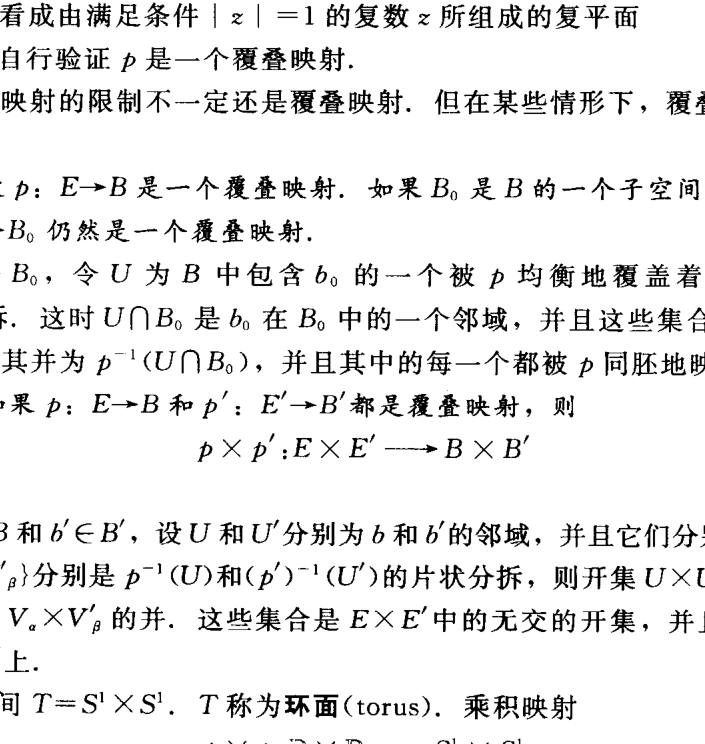
\includegraphics[width=0.5\textwidth]{image/fig-53-4.png}
\caption{$p\times p\colon\mathbb{R}^{2}\to T$.}
\label{figure:ch09-fig-53-4}
\end{figure}

积空间 $S^{1}\times S^{1}$ 是 $\mathbb{R}^{4}$ 的子空间, 因而难于形象化, 图中画的环面并不是 $S^{1}\times S^{1}$, 而是大家熟知的 $\mathbb{R}^{3}$ 中的轮胎状曲面 $D$, 它是用一个 $xz$ 平面上中心为 $(1,0,0)$、半径为 $\frac{1}{3}$ 的圆周 $C_1$ 绕着 $z$ 轴旋转而得到的. 不难看出, $S^{1}\times S^{1}$ 与曲面 $D$ 之间的一个同胚. 令 $C_2$ 表示 $xy$ 平面上以原点为中心、以 $1$ 为半径的圆周, 定义映射 $f\colon C_1\times C_2\to D$, 使得 $f(a,b)$ 是当我们绕 $z$ 轴旋转 $C_1$, $C_1$ 的中心正好到达 $b$ 时, $C_1$ 上的点 $a$ 到达的那个点 (参见图 \cref{figure:ch09-fig-53-5}). 可以想象得到, $f$ 是 $C_1\times C_2$ 与 $D$ 之间的一个同胚. 如果愿意的话, 读者可以写出 $f$ 的方程, 并且直接验证 $f$ 是连续的既单且满的映射. ($f$ 的连续性可以根据 $C_1\times C_2$ 的紧致性推出.)

\par
\begin{figure}[htbp]
\centering
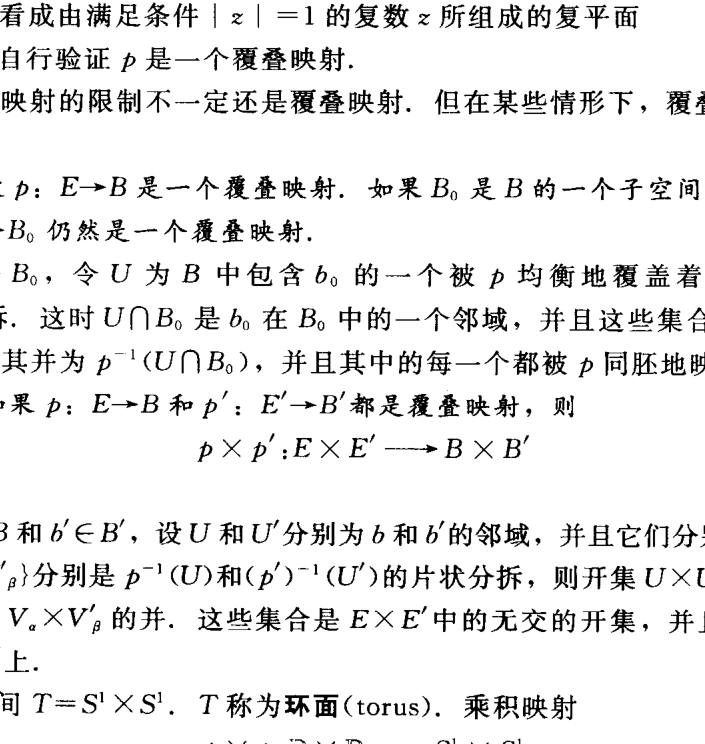
\includegraphics[width=0.5\textwidth]{image/fig-53-5.png}
\caption{环面作为旋转曲面.}
\label{figure:ch09-fig-53-5}
\end{figure}

\begin{example}
\label{example:ch09-sec53-5}
考虑前例中的覆叠映射 $p\times p$. 设 $b_0$ 表示 $S^{1}$ 中的点 $p(0)$, $B_0$ 表示 $S^{1}\times S^{1}$ 的子空间
\[
B_{0}=(S^{1}\times b_{0})\cup(b_{0}\times S^{1}),
\]
则 $B_0$ 是在一点处相交的两个圆周的并, 我们常称之为\textbf{8 字形空间}(figure-eight space). 空间 $E_0=p^{-1}(B_0)$ 是画在图 \cref{figure:ch09-fig-53-4} 中的"无限网格"
\[
E_{0}=(\mathbb{R}\times\mathbb{Z})\cup(\mathbb{Z}\times\mathbb{R}).
\]
$p\times p$ 的限制映射 $p_0\colon E_0\to B_0$ 便是一个覆叠映射.

这个无限网格是 8 字形空间的覆叠空间之一, 稍后我们还要讨论其另外的覆叠空间.
\end{example}

\begin{example}
\label{example:ch09-sec53-6}
考虑覆叠映射
\[
p\times i\colon\mathbb{R}\times\mathbb{R}_{+}\longrightarrow S^{1}\times\mathbb{R}_{+},
\]
其中 $i$ 是 $\mathbb{R}_{+}$ 上的恒等映射, $p$ 是定理 \cref{theorem:ch09-sec53-53-1} 中的映射. 如果我们取从 $S^{1}\times\mathbb{R}_{+}$ 到 $\mathbb{R}^{2}-\boldsymbol{0}$ 的标准同胚, 即将 $x\times t$ 映为 $tx$ 的同胚. 复合映射便给出了一个用上半开平面覆叠穿孔平面的覆叠映射
\[
\mathbb{R}\times\mathbb{R}_{+}\longrightarrow\mathbb{R}^{2}-\boldsymbol{0}.
\]
这个覆叠映射画在图 \cref{figure:ch09-fig-53-6} 中, 它在研究复变函数时作为复对数函数的 Riemann 面出现.
\end{example}

\par
\begin{figure}[htbp]
\centering
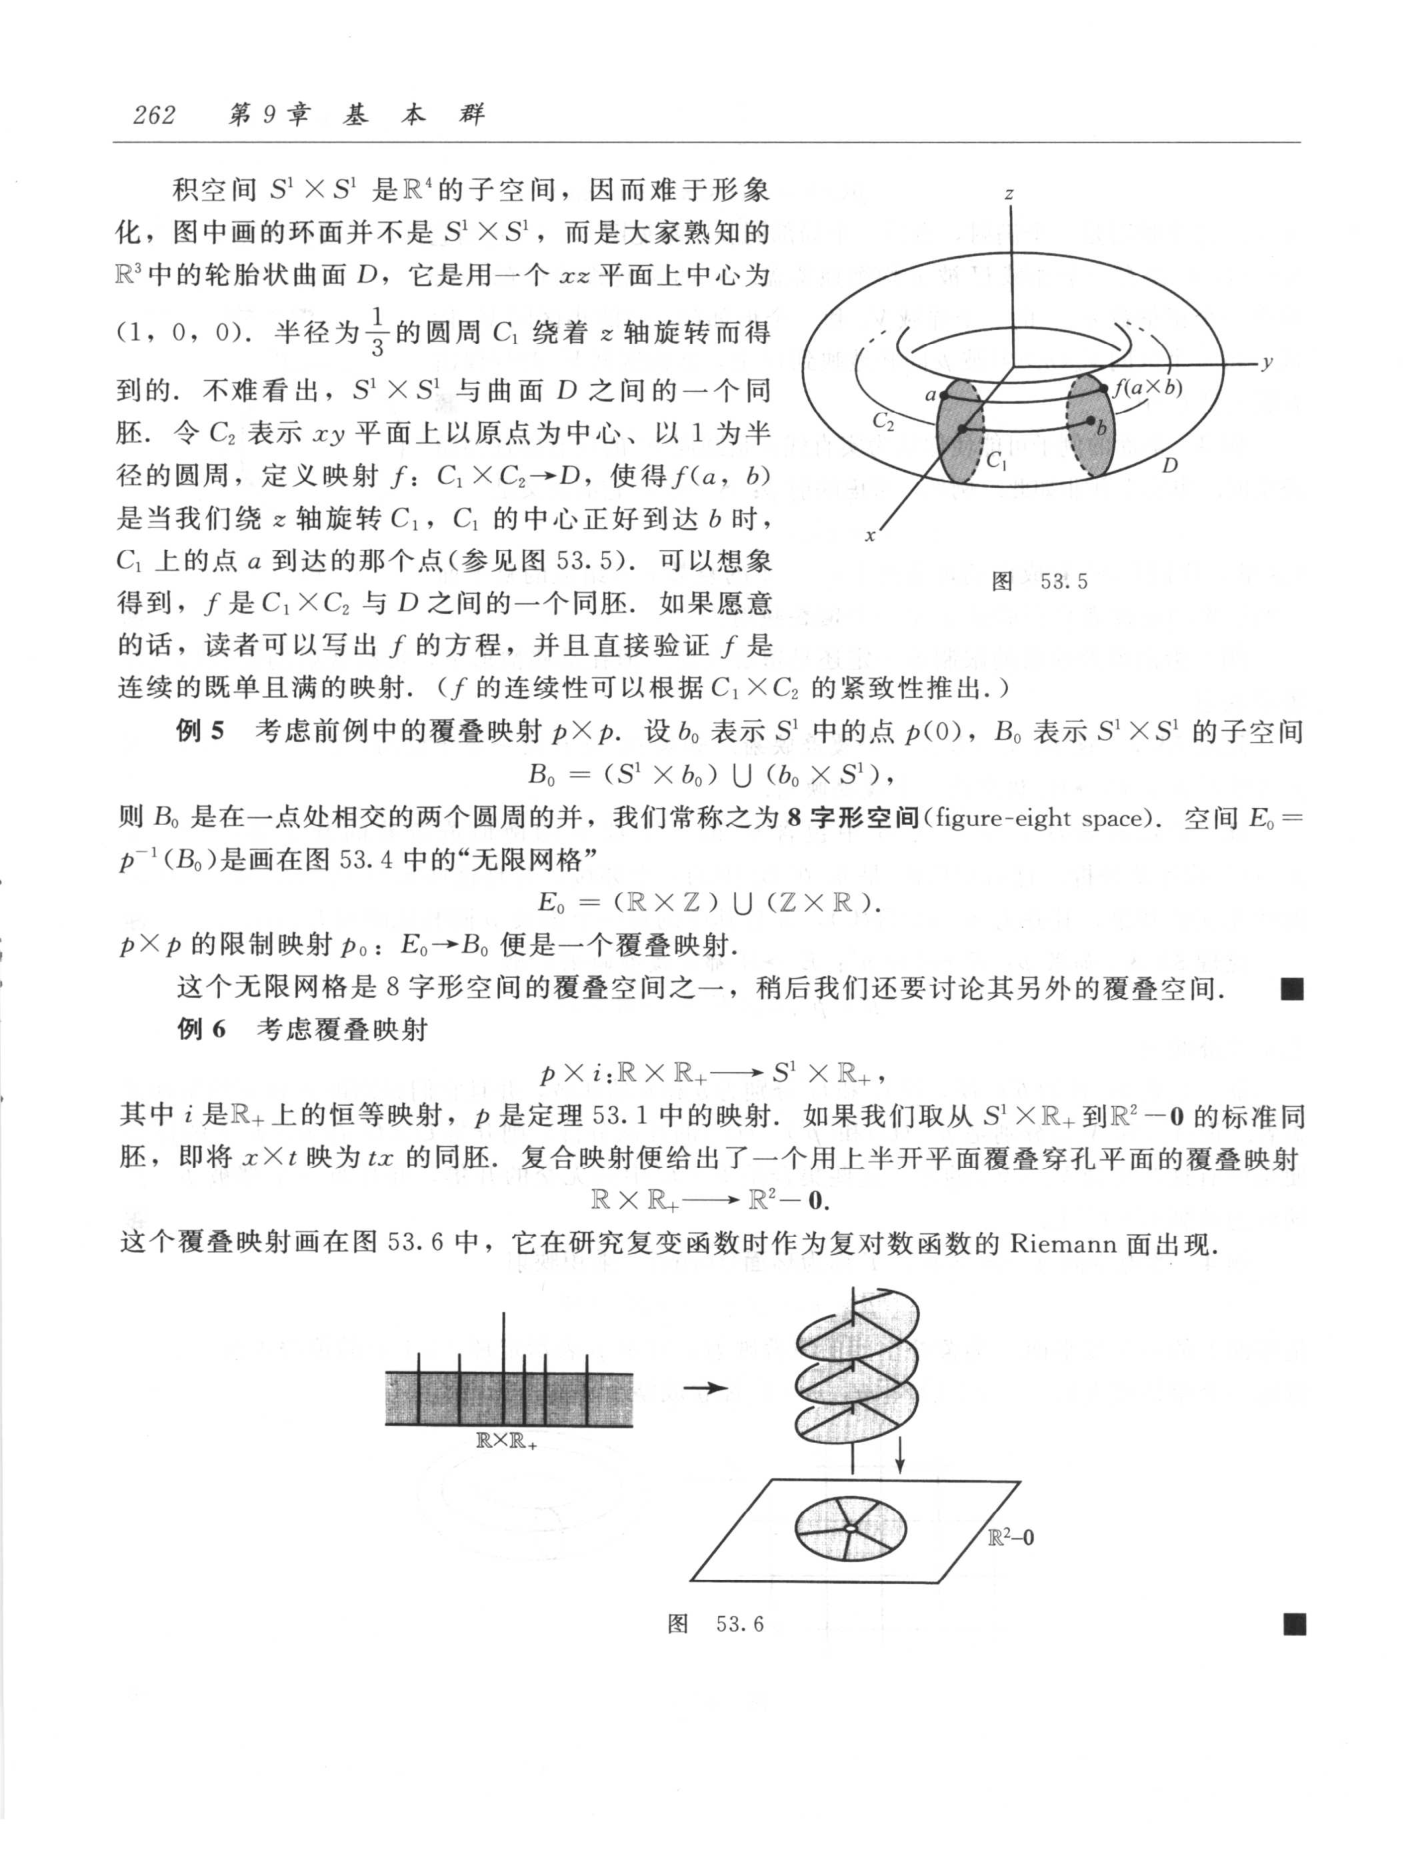
\includegraphics[width=0.5\textwidth]{image/fig-53-6.png}
\caption{穿孔平面的覆叠空间.}
\label{figure:ch09-fig-53-6}
\end{figure}
